\fancyhead[LO]{{\scriptsize {\FA \ }我们最幸福 {\FA } 故乡里的陌生人}}%奇數頁眉的左邊
\fancyhead[RO]{{\tiny{\textcolor{Gray}{\FA \ }}}\thepage}
\fancyhead[LE]{{\tiny{\textcolor{Gray}{\FA \ }}}\thepage}
\fancyhead[RE]{{\scriptsize {\FA \ }我们最幸福 {\FA } 故乡里的陌生人}}%偶數頁眉的右邊
\fancyfoot[LE,RO]{}
\fancyfoot[LO,CE]{}
\fancyfoot[CO,RE]{}
\chapter*{19 {\FA } 故乡里的陌生人}
\addcontentsline{toc}{chapter}{\hspace{5mm}19 {\FA } 故乡里的陌生人}
\begin{figure}[!htbp]
\centering
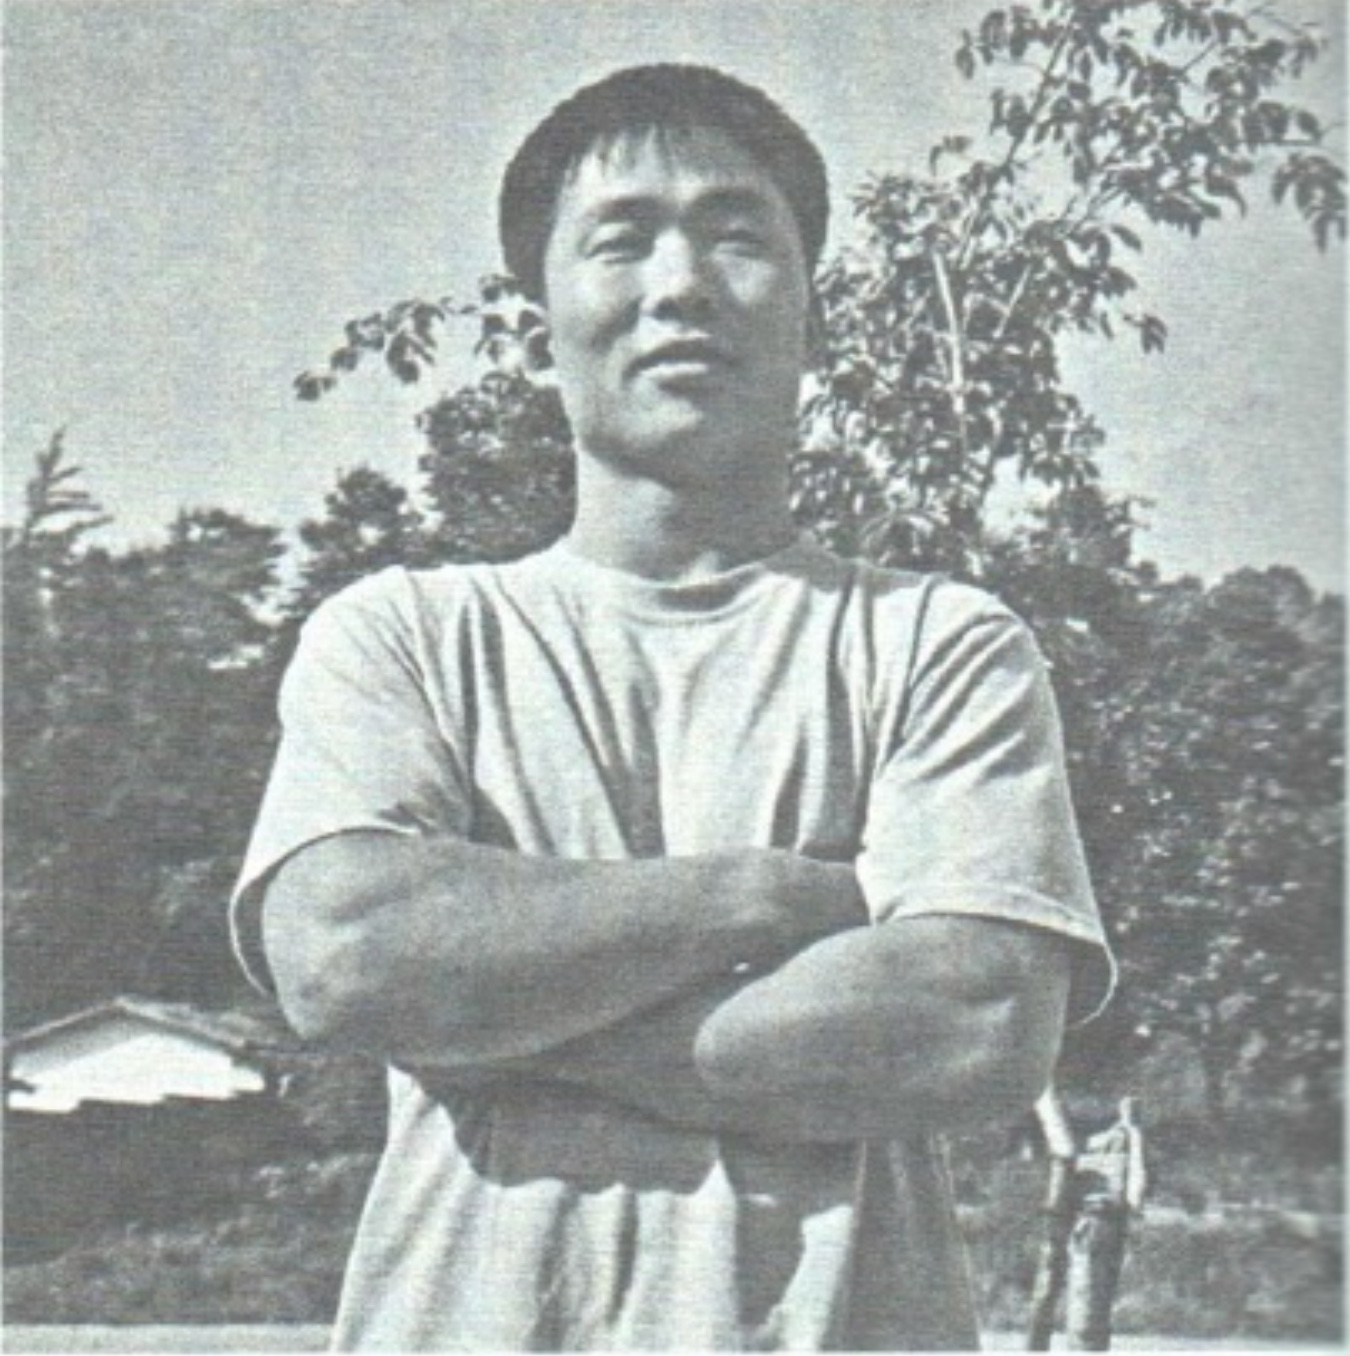
\includegraphics[width=6cm]{./Chapters/Images/19.jpg}
\caption*{2004年的金赫}
\end{figure}


在南韩最看重的质素是──个子高、皮肤白、财富、声望、学位、名牌服装、流利的英语──而所有的这些,都是那些新抵达的脱北者所缺乏的,这造成了在这些脱北者当中普遍的自卑,例如玉熙。其实南韩人50年前也好不到哪里去,但是当北朝鲜人提醒南韩人的过去时,他们更愿意选择忘记。脱北者也意识到一个令他们惊骇的事实──南韩人害怕金正日政权的垮台,那将导致在他们的国家里泛滥着2300万人,要吃的、要住的。声称所有朝鲜人都渴望着他们的离散亲属,是政治上正确的\footnote{“统一是我们的渴望,做梦都想。”},但是有些人却对这些的未来感到恐怖。首尔的智库也定期的发布报告,估计统一的费用,这个数字通常介于3000亿美元至18000亿之间。生于战后多年的年轻人,对于失去的另外一半的朝鲜也没什么伤感。他们宁愿忽略,在北边张牙舞爪的这个赤贫的、装备有核武的独裁政权。纵观他们繁忙的生活,有着发达国家最长的工作时间,他们疯狂的玩乐、他们驾着现代车狂飙、他们听着iPod的咆哮其它的都很容易被忘记。\\

对于政府提供的所有支持,脱北者们能够感到这是南韩人对他们的可怜、害怕、歉疚和尴尬。这样感情复杂的欢迎,让他们觉得在自己的祖国里就像是陌生人。\\

金医生本没什么意愿逃亡南韩。当她于1999年跨过图们江时,她的目的地只是中国。她计划按照父亲死前写的名字和最后知道的地址找到在中国的亲戚。她想他们会帮她找些事情做。她可以吃的好些,恢复体力,然后再给儿子存点钱。最终,她还是要回清津,回医院工作的。虽然吃不饱,同劳动党也发生争执,但是她仍然认为自己亏欠给她以教育的国家。\\

当真的跨越国境后,金医生来到中国的第一个小时,看见一大碗给狗吃的混着肉的白米饭,她的决心就动摇了。每过一天,就有新的见识,也让她更深一步对自己被灌输的谎言感到愤怒。所有事物都在驱使她与自己的祖国、曾经的信仰渐行渐远,直到再也无法回头。\\

当她推开农舍的大门时,那只狗开始拼命的狂吠,随后走过来它的主人。他们都是朝鲜族人,一个老妇和她成年的儿子。他们从金医生冻结的衣服和憔悴的神情就知道是新到的难民。他们请她进屋,给了她干衣服和一顿热食。这些陌生人本可以把她以几百块的价格当新娘卖了──她才34岁,还比较吸引人──但是相反,他们却收留了她两周,并帮她找到了父亲的亲戚。在亲戚那也是,她受到了让人惊讶的慷慨招待。她那些从未谋面的亲戚立刻把她当家人收留了下来。\\

起先,金医生毫无困难的融入其它朝鲜族人。她还学了一点点中文。她在一家饭店找了份工作,为工人做盒饭。但是到了2000年,中国警方加强了搜捕脱北者。金医生被抓了三次。每次都是亲戚们贿赂当地的警官,把她放了出来。在最后一次被释放后,金医生认为继续待在中国东北太危险了。她坐上火车去北京找工作。称自己是来自于延边的朝鲜族,她应征了一个需要说朝鲜语的保姆工作。\\

金医生的雇主是个在职母亲,一个南韩的教授带着5岁的孩子来中国进行为期1年的学术交流。金医生很喜欢这个教授,籍此她也有机会住在舒适的公寓里帮她带孩子。她证明自己是个非常称职的保姆和管家。在1年的交流即将届满时,这个教授建议她随他们全家去南韩。很多富裕的南韩家庭都雇有中国朝鲜族作为保姆。\\

因此,金医生觉得别无选择只有坦白。她把自己的故事全盘托出──离婚还有失去儿子监护权,父亲在金日成死后也自杀了,多年的食不果腹,医院里垂死的孩子。\\

“我的天啊,你是个医生!”这个教授惊呼道。两个女人抱头痛哭。“如果我知道,我早就对你另眼相待了”\\

“如果你早知道,我就没有机会给你工作。我需要这份工作。”\\

坦白很快终结了金医生的保姆生涯,但是教授言出必行。她允诺无论如何都要带她去南韩。走了几个月后,她让一个中间人联系到了金医生。\\

在2002年3月,金医生抵达仁川机场,心满意足的开始了新的生活。但是这种感觉没有持续多久。金医生被一个在教堂认识的人说服,将2万美元的安置费投入一个传销活动,就是向熟人兜售肥皂和化妆品。金医生在自己的培训计划中没有学习如何识破骗局;销售的本质其实就是一个金字塔的骗术,她因此损失了几乎所有的政府给的钱。之后,她又遭到另一个挫折:她得知南韩政府不承认她的医学教育。如果想行医,她就必须从头开始,申请医学院,再自行支付学费,因为她年纪太大而得不到政府的奖学金。金医生沮丧至极。7年的医学院学习,8年的行医经历,这一切归为零。她变得自艾自怨。内心里对于离弃北朝鲜也感到隐隐的愧疚,甚至还想到了自杀。\\

当我2004年遇到金医生的时候,我问她是不是对于来到南韩感到后悔。\\

“如果我知道我现在所知道的这些,我是不会来的。”她回答道,这是我所遇见的脱北者里唯一这样承认的,虽然我怀疑很多其它人也有类似想法。我也禁不住注意到金医生看上去仍然像个北朝鲜人。她的头发梳到脑后,用一条天鹅绒丝带扎起来,她仍然用60年代印染彩色电影里那种明红色的口红涂抹她那弓形的嘴唇。她让我想到了在平壤城区见到的劳动党党员。\\

几年后,当我又遇见她,她已经完全脱胎换骨了。2007年的夏天,我都不敢认走进首尔一个新开张的日本餐厅的那个时髦女人了。她留了一个蓬松的披肩发,穿着蓝色牛仔裤,耳朵上吊着长长的耳环。\\

“我已经厌倦了俗气的北朝鲜装扮。”她告诉我。\\

她看上去年轻多了,像个学生,实际上她也确实是。在同南韩卫生部抗争了多年后,她忍受着巨大痛苦,并且在40岁的时候开始了她的4年医学培训。她同那些几乎小她20岁的同学们住在宿舍。关于她的学习,她告诉我,很艰难,不是因为她在北朝鲜接受的培训使她准备不足,而是在南韩医学院里用太多的英文术语,而她对这些完全不熟悉。她学过的唯一外语就是俄语。然而,这个过程让她好像得以重生。在毕业后,她计划重操旧业,这次她专注于老年保健。她的母亲因老年痴呆症,死得很痛苦。金医生还梦想开个护理中心,甚至可能是连锁的护理中心。她希望有朝一日,当北朝鲜政权垮台后,她可以将南韩照料年长者的观念带回清津。也许这是白日梦,但是这帮她在自己的过去和现在建立起一个桥梁,而且缓解了自己对所辜负的那些人的负罪感。\\

不幸的是,脱北者群体往往是些麻烦缠身的人。很多人离开不仅仅是因为饥饿,而是因为在家待不下去。而且他们的麻烦也常常会如影相随,即使跨过了边界。\\

这在金赫身上体现的尤为突出。他19岁的时候到了南韩,他和以往一模一样──贫穷、矮小、无家可归,也没有家庭或亲戚朋友在生活上帮帮他。\\

金赫于2000年6月从第十二劳动营感化所被释放。此时,他因营养不良身体非常虚弱,以至于走上个百多米就要休息一阵子。在恢复到能进行下一步行动前,他一直待在一个朋友家。起先,金赫计划从新开始他走私的营生,然而劳动营的经历彻底碾碎了他的信心。18岁了,金赫已经完全没有了那种十几岁时可以为所欲为、不惧艰险的护身符。他不想再次被抓;他不想再挨打。他对于逃跑已经厌倦了。他对北朝鲜也没什么眷恋了;如果他逃去中国,他会一直被追捕。他认为唯一的机会就是逃往南韩。他完全不知道怎么才能到那儿,但是他听说过一些南韩的传教士会帮助像他这样的无家可归者。于是,当他2000年平安夜最后一次度过图们江后,他径直就去找教堂。\\

作为菲律宾之后亚洲第二大天主教国家,南韩派遣的传教士遍布亚洲,非洲,中东,传播着福音及提供人道主义援助。与大多数南韩人对脱北者矛盾的态度不同的是,这些传教士积极帮助北朝鲜人脱困。其时,数以千计的南韩传教士──有时候兼有韩裔美国传教士──成群结队来到中国东北地区,在那里他们很小心低调以免触怒中国当局,在一些私人住宅里运作着一些小的、未经注册的地下教堂。\\

在夜间,他们那红色的霓虹灯十字架在黑暗的乡村里透着一股阴森。其它的一些北朝鲜人的安全之所只是口口相传。由于联合国难民事物高级专员和一些主流的非政府组织无法公开违反中国反对为北朝鲜人提供庇护的法律,这些传教士就通过提供食物和庇护所给难民填补了这些重要的空白。\\

金赫在沈阳,中国东北最大的城市,找到了一个教堂。这个教堂是由一个开家具厂的南韩商人运营,听说这里能提供联系和资金安排一个安全通道去南韩。\\

“我想了解基督教。”金赫撒谎道。\\

金赫把自己交给了循规蹈矩的日子。他和一些其它的脱北者每天早晨5点起床,祈祷。之后是早餐,锻炼,学习圣经,晚餐,然后9点就寝前还要祈祷一次。除了周末,日子每天都这样,周末他们偶尔踢踢足球。像其它他这个年纪的北朝鲜人,金赫从未听说过基督耶和华。清津的教堂在他出生的几十年前就关闭了;老一代的人仍然会祈祷,但是都是私下里。在小学的读物里,也几乎没有提及任何关于基督教的事情,即使有些,那些传教士也都是以恶棍的面目出现,奸诈且残忍。金赫也对基督教心存芥蒂。他认为南韩教堂迫使他吞进他们的教化以换取食物和住所。然后另一方面,他觉得有点愧疚于自己假装成为信众来欺骗他们。慢慢的他的态度有所软化。在过了一段时间,当喃喃的念着那些祈祷词时,他觉得一种安逸,一种自年幼背诵关于金日成的诗歌以来从未享有过的安逸,以及一种高于对自身的信任。\\

只在此时,当他说“Uri Abogi”我们的天父时,他意指上帝,而不是金日成,当他说圣子时,他意指的是基督,而不是金正日。\\

在教堂待了5个月后,教长建议金赫现在是时候更进一步了。教堂现在处于中国警方的严密监控之下,他们担心这些难民的安全。这个人给了金赫1000元人民币并要求他带领一队难民前往蒙古边界。从那里,他们可以去南韩。\\

如果宋女士拿着伪造的护照坐飞机的线路是贵宾头等舱的话,那么蒙古线路就是统舱散席了。但是对于没有钱的人来说,这是最好的离开方式。不像中国人,蒙古人允许南韩驻乌兰巴托──蒙古首都,的大使馆接收脱北者。实际上,如果北朝鲜人想方设法溜出中国进入蒙古,他们都会被蒙古的边境警察逮捕,之后就会移交、驱逐──去南韩。在蒙古被捕实际上就等于一张去首尔的机票。因此,真正意义上蒙古成了北朝鲜人前往南韩的地下铁路在线的主要补给站。\\

金赫和其它一些难民乘火车抵达了二连浩特,这是前往蒙古边境的最后一个中国城市,一个骆驼,牛羊多过其人口的沙漠前哨地。他们一行六个北朝鲜人,包括一个3岁,一个10岁的男孩,他们的父亲已经在南韩了。计划是在一个安全地点同另一组,乘另外一趟列车从大连来的北朝鲜人汇合。另一组里有个人熟悉地形,会带领他们穿过边界。\\

但是出了岔子。还在火车上的时候,金赫接到个令人心悸的电话,通知他另外一组人被捕了。他们这组人别无选择──现在回头为时已晚。他们不能去那个安全地点,因为那里可能已经处于监视之下。他们不得不丢掉手机,因为那可能会向警方暴露他们的行踪。金赫和其它的成年人们商量着。他们曾被简单的交代过行进路线,还有一张手绘的地图。最后,他们决定无论如何也要自行前往蒙古边界。\\

这些人躲在二连浩特火车站附近直至晚上9点,等着夏日长昼最后一缕光线褪去之后,他们就可以乘着夜色赶路。他们曾被告知沿着向北通往乌兰巴托的主铁路线,用铁轨当向导,之后要穿过一个分割两国边界的220公分高的铁丝围栏。\\

从二连浩特火车站到第一道边境围栏只有区区8公里,从那里再走2公里就到了蒙古第一个观察哨,在那里他们要向当局投降。他们应该能在天亮之前走到那里,但是沙漠到了夜间很容易让人迷路──只有星星可以引导他们,而且一路上遍布荆棘,岩石和深褐色的沙土。大人们不断的因为走哪条路而发生着争吵。\\

他们应该沿着铁轨向东还是向西呢?他们选择了向东,后来证明是大错特错。边境线先是向东北延伸,之后突然向北急拐;就这样他们一直沿着与国境线平行的方向走,而不是靠近国境线并穿越过去。当天蒙蒙亮的时候,他们意识到了错误。戈壁沙漠上的气温一下子窜到了32度多。当他们改变方向,发现勾勒出两国边界的围栏,并穿过去的时候,时间已经来到了下午很晚的时候。他们的鞋被崎岖的地表磨得破破烂烂,很多人的脚都在流血,一个个都被晒伤。他们带的6升水也早就喝完。金赫和其它人轮流背着3岁的孩子,但是当10岁的孩子跟不上时,他们也无能为力只能拖着他走。最终他们发现了个位于一个小水塘附近废弃的一间小木屋。当金赫跑去取水的时候,一个女人待在孩子身边。当他回来的时候,他听见这个女人的恸哭。孩子死了。\\

蒙古的边境警察在晚上发现了这些北朝鲜人。出现死亡的孩子让这个案子变得复杂起来。法医需要核实死亡是由脱水导致的,而不是谋杀。对他们的调查延续了10周,在此期间金赫和其它成年人都被关押在蒙古的监狱中。对于金赫刚刚开始的自由世界的生活,这可不是个好兆头。\\

金赫于2001年9月14日,乘坐从乌兰巴托起飞的航班抵达南韩,同行的还有一打其它的脱北者。仁川国际机场移民局官员在他于蒙古获颁的临时护照上盖章后对金赫说,“欢迎来到南韩”,此时金赫几近虚脱。\\

同很多脱北者一样,金赫的的欣喜很快就消失了。由于曾经被关进监狱,对他的聆讯进行的异常折磨人。南韩政府对脱北者中的犯罪分子越来越警惕。之后,正如他想象的那样,他被释放,送入统一院的营地待了1个月。他忍受不了被限制自由。\\

金赫的个性在南韩同在北朝鲜一样成为障碍。他易怒。他对当局不感冒。他不能安静的坐会儿。在一个崇尚高大的社会里,他的身高也成了不利因素。他的腿发育不全,他的头相对于他的身体也显得很大──这是对于那些在身体发育时,没有足够食物的人典型的身体特征。当没有营养时,身体就会引导资源优先供应给头部和躯干,而且牺牲四肢。在饥荒相关文献中,这种症状成为“发育迟缓”。在2003年由世界粮食计划署和联合国儿童基金会发起的一项研究中发现,42\%的北朝鲜儿童由于这个原因,身体受到永久性的损伤。\\

当我们2004年第一次会面时,金赫住在扶余,首尔以南2个小时车程的一个省会城市。在那里周围没什么脱北者,也没人帮他安定下来。他说他的神经受不了大城市的噪音和拥堵。他一文不名,2万美元的安置费用几乎一到手就损失殆尽。他把钱给了一个声称可以找到哥哥的中间人。在被愚弄了近1年后,金赫估计自己的哥哥可能已经死了。“我哥哥差不多有180公分高。他很难活下来。”他告诉我。身材矮小的一个好处就是你需要的食物会少些。\\

金赫的工作换了一个又一个。有段时间他送冰激凌,之后他发现自己公司的南韩雇员薪水更高,于是他就生气的辞职了。他参加了一个汽车机修工的培训,之后作为实习人员做了几个月,但是也没有坚持下来。之后,他又认为自己的真正命运是成为一个职业的拳击手,但是当他去首尔的一家拳击馆后,因为太矮,而被拒绝了。这严重的打击了他的自尊心,使得他开始担心自己永远找不到女友。\\

他孤独至极。他同生人沟通很难。如果南韩人很同情他,他就觉得他们很有优越感。即使他憎恨北朝鲜政权,当南韩人批评它的时候,他发现自己会为它辩护。这是脱北者之中很普遍的困境。\\

一些南韩基本的礼仪也让他无所适从。北朝鲜人没有习惯与陌生人闲扯几句,如果有人这么做,会让人侧目的。无论何时当金赫出门时,邻居随意的一句招呼都会吓他一跳。作为响应,他只是转开视线或者有时候皱皱眉。\\

“我不知道当人们同你讲几句话的时候,你该如果应答。我不明白怎样才能同邻居们或者那些帮助过我的人建立起友谊。”金赫后来回忆起在南韩第1年的那些社交过失时会哈哈大笑。\\

当我在2008年再次见到他的时候,他已经搬去首尔并被一家学院录取,希望能获得历史和商业上的学位。那时他26岁了。虽然令人遗憾的还没找到女朋友,但是他有了很多朋友,包括一个来自茂山刚刚抵埠的表亲。带领一个生手熟悉各方面情况的过程也增强了他的自信心。他告诉我,他最近遇到一个在大学附近开了间私人英语学校的人。他们就在街头攀谈了起来。没有逃走,相反金赫告诉这个人他是脱北者,而这个人则邀请他免费去他的学校学习。\\

他融入了。\\
